\documentclass[aip,jcp,reprint,noshowkeys,superscriptaddress]{revtex4-1}
\usepackage{graphicx,dcolumn,bm,xcolor,microtype,multirow,amsmath,amssymb,amsfonts,physics,mhchem,xspace,subfigure}

\usepackage[utf8]{inputenc}
\usepackage[T1]{fontenc}
\usepackage{txfonts}

\usepackage[
	colorlinks=true,
    citecolor=blue,
    breaklinks=true
	]{hyperref}
\urlstyle{same}

\definecolor{darkgreen}{HTML}{009900}
\usepackage[normalem]{ulem}
\newcommand{\sphi}[1]{\hat{{\bf S}}_{#1}}
\newcommand{\overlap}[2]{\langle #1 | #2 \rangle}
\newcommand{\matelem}[3]{\langle #1 | #2 | #3 \rangle}
\newcommand{\deriv}[3]{\frac{\partial^{#3} #1}{\partial {#2}^{#3}}}
\newcommand{\bd}[1]{{\bf {#1}}}
\newcommand{\br}[0]{{\bf {r}}}
\newcommand{\bs}[0]{{\bf {s}}}
\newcommand{\dr}[1]{\text{d}{\bf {#1}}}
\newcommand{\psiex}[0]{\Psi^{\text{ex}}}
\newcommand{\energyex}[0]{E^{\text{ex}}}

\begin{document}	

\title{On the general mapping between effective two-electron interaction and Jastrow factors.}

\author{Emmanuel Giner}
\email{emmanuel.giner@lct.jussieu.fr}

\begin{abstract}
blabla

\end{abstract}

\maketitle
\section{Position of the problem: the cusp of the helium atom}
Consider the Hamiltonian of He atom: 
\begin{equation}
 \label{eq:h_he}
 \begin{aligned}
 H = &-\frac{1}{2} \sum_{i=1}^2 \bigg(\deriv{}{r_i}{2} + \frac{2}{r_i} \deriv{}{r_i}{} + \frac{2 Z}{r_i}\bigg) \\
     &-\bigg( \deriv{}{r_{12}}{2} + \frac{2}{r_{12}} \deriv{}{r_{12}}{} -\frac{1}{r_{12}}\bigg) \\
     &-\bigg( \frac{\bd{r_1}}{r_1} \cdot \frac{\bd{r_{12}} }{r_{12}}  \deriv{}{r_1}{} + 
              \frac{\bd{r_2}}{r_2} \cdot \frac{\bd{r_{21}} }{r_{21}}  \deriv{}{r_2}{} \bigg).
 \end{aligned}
\end{equation}
The exact wave function $\psiex(\bd{r_1},\bd{r_2})$ must satisfy the Schrodinger equation for all points $(\bd{r_1},\bd{r_2})$, which means that 
\begin{equation}
 H \psiex(\bd{r_1},\bd{r_2}) = \energyex \psiex(\bd{r_1},\bd{r_2}) \quad \forall (\bd{r_1},\bd{r_2}).
\end{equation}
When looking at $r_{12}\approx 0$, the terms multiplying $\frac{1}{r_{12}}$ must remain finite, which translates into 
\begin{equation}
 \bigg( \frac{2}{r_{12}} \deriv{}{r_{12}}{} -\frac{1}{r_{12}}\bigg) \psiex(\bd{r_1},\bd{r_2})  = c,\quad c<\infty 
\end{equation}
which translates into
\begin{equation}
 2 \deriv{\psiex(\bd{r_1},\bd{r_2})}{r_{12}}{} -\psiex(\bd{r_1},\bd{r_2})  = c\times r_{12}. 
\end{equation}
At $r_{12}=0$, one obtains the famous cusp condition
\begin{equation}
 \deriv{\psiex}{r_{12}}{}\Bigr|_{r_{12}=0} = \frac{1}{2} \psiex(r_{12}=0). 
\end{equation}
%Nevertheless, imposing $c=0$ is just a choice, as long as $c<\infty$ one can satisfies the Schrodinger equation. 
%In the next section, we will focus on imposing a finite value. 

\section{Wave function with a Jastrow factor}
Let us assume now that we have an approximate wave function $\Psi(r_{12)}$ which is obtained from a Jastrow factor $f(r_{12})$ and a wave function $\psi(r_{12})$
\begin{equation}
  \Psi(r_{12)} = e^{f(r_{12})} \phi(r_{12}). 
\end{equation}
Let us plug such a wave function in the previous equation
\begin{equation}
 \begin{aligned}
 & \bigg( \frac{2}{r_{12}} \deriv{}{r_{12}}{} -\frac{1}{r_{12}}\bigg) e^{f(r_{12})} \phi(r_{12}) \\
 = & e^{f(r_{12})} \bigg[ \frac{2}{r_{12}} \deriv{\phi}{r_{12}}{} - \left( \frac{1}{r_{12}} - \frac{2}{r_{12}}\deriv{f}{r_{12}}{} \right) \phi(r_{12}) \bigg].
 \end{aligned}
\end{equation}
Therefore, by multiplying by $e^{-f(r_{12})}$ one obtains a similarity transformed Hamiltonian and therefore 
\begin{equation}
 \label{eq:eff_h}
 \begin{aligned}
 & e^{-f(r_{12})} \bigg( \frac{2}{r_{12}} \deriv{}{r_{12}}{} -\frac{1}{r_{12}}\bigg) e^{f(r_{12})} \phi(r_{12}) \\ 
=& \frac{2}{r_{12}} \deriv{\phi}{r_{12}}{} - \left( \frac{1}{r_{12}} -  \frac{2}{r_{12}}\deriv{f}{r_{12}}{} \right) \phi(r_{12}) \\
=& \frac{2}{r_{12}} \deriv{\phi}{r_{12}}{} - \frac{1}{r_{12}} \left( 1-  2 \deriv{f}{r_{12}}{} \right) \phi(r_{12}). 
 \end{aligned}
\end{equation}
As before, one imposes that such quantity remains finite at $r_{12} = 0$, which translates into
\begin{equation}
 2 \deriv{\phi}{r_{12}}{} = \left( 1-  2 \deriv{f}{r_{12}}{} \right) \phi(r_{12}). 
\end{equation}
Now let us impose that $\phi(r_{12})$ is cusp-less, \textit{i.e.}
\begin{equation}
 \deriv{\phi}{r_{12}}{} = 0, 
\end{equation}
this translates into 
\begin{equation}
 \deriv{f}{r_{12}}{} = \frac{1}{2}, 
\end{equation}
or 
\begin{equation}
 f(r_{12}) = f(0) + \frac{1}{2} r_{12} + \hdots 
\end{equation}
Therefore, a Jastrow factor of form $e^{\alpha + \frac{1}{2} r_{12}}$ can fulfill the conditions. 

\section{Link with an effective non divergent interaction}
Let us rewrite Eq. \eqref{eq:eff_h} as 
\begin{equation}
 \label{eq:eff_h}
 \begin{aligned}
 & e^{-f(r_{12})} \bigg( \frac{2}{r_{12}} \deriv{}{r_{12}}{} -\frac{1}{r_{12}}\bigg) e^{f(r_{12})} \phi(r_{12}) \\ 
 =& \frac{2}{r_{12}} \deriv{\phi}{r_{12}}{} - \frac{w(r_{12})}{r_{12}} \phi(r_{12}),
 \end{aligned}
\end{equation}
with 
\begin{equation}
 \label{eq:dev_wr12}
 w(r_{12}) =  1-  2 \deriv{f}{r_{12}}{}.
\end{equation}
This equation can be seen as a piece of an effective Hamiltonian of the form of Eq. \eqref{eq:h_he} but where the regular coulomb interaction $1/r_{12}$ would be replaced by $w(r_{12})/r_{12}$. 

Therefore, one can have a \textit{quantitative and constructive} mapping between a general two-electron interaction, and a general Jastrow factor. 
One can notice that one can choose $w(r_{12})$ such that 
\begin{equation}
 \label{eq:wr12}
 \lim_{r_{12}\rightarrow 0} \frac{w(r_{12})}{r_{12}} < \infty,
\end{equation}
which helps therefore in designing a Jastrow factor which makes the effective interaction non divergent. 


\section{The case of the long-range interaction of RS-DFT}
As a special case of Eq. \eqref{eq:wr12}, one can choose the long-range interaction of RS-DFT, which is nothing but imposing 
\begin{equation}
 w(r_{12}) = \text{erf}(\mu r_{12}). 
\end{equation}
Therefore, thanks to Eq. \eqref{eq:dev_wr12}, we can obtain the form of the Jastrow factor which would give an effective interaction of of the form 
\begin{equation}
 \frac{w(r_{12})}{r_{12}} = \frac{\text{erf}(\mu r_{12})}{r_{12}}. 
\end{equation}
This translates into 
\begin{equation}
 1-  2 \deriv{f}{r_{12}}{} = \text{erf}(\mu r_{12}), 
\end{equation}
which is a differential equation which can be integrated (thank God for Wolfram Alpha) and gives
\begin{equation}
 \label{eq:def_f}
 f(r_{12};\mu) = \frac{1}{2}r_{12}\bigg( 1 - \text{erf}(\mu r_{12})  \bigg) - \frac{1}{2\sqrt{\pi}\mu}e^{-(r_{12}\mu)^2} + cst
\end{equation}
where $cst$ is a constant. Here we take the $cst$ such that $\lim_{\mu \rightarrow \infty} f(r_{12};\mu) = 0$ in order to have a Jastrow factor becoming $1$ at large $r_{12}$. 


\section{Study of the Jastrow factor as a function of $\mu$ and $r_{12}$}
Let us call the $\mu$-dependent Jastrow factor $J(r_{12};\mu)$
\begin{equation}
 J(r_{12};\mu) = \text{exp}(f(r_{12};\mu))
\end{equation}
with of course 
\begin{equation}
 f(r_{12};\mu) = \frac{1}{2}r_{12}\bigg( 1 - \text{erf}(\mu r_{12})  \bigg) - \frac{1}{2\sqrt{\pi}\mu}e^{-(r_{12}\mu)^2}.
\end{equation}
\subsection{Some limits in terms of $\mu$}
\subsubsection{$\mu \rightarrow \infty$}
In that case one has
\begin{equation}
 \lim_{\mu \rightarrow \infty} \text{erf}(\mu r_{12}) = 1,
\end{equation}
which means that the effective interaction in that limit is the full Coulomb interaction
\begin{equation}
 \lim_{\mu \rightarrow \infty} \frac{\text{erf}(\mu r_{12})}{r_{12}} = \frac{1}{r_{12}}.
\end{equation}
Regarding now the function $f(r_{12};\mu)$, one has 
\begin{equation}
 \lim_{\mu \rightarrow \infty} \frac{1}{2}r_{12}\bigg( 1 - \text{erf}(\mu r_{12})  \bigg) = 0,
\end{equation}
\begin{equation}
 \lim_{\mu \rightarrow \infty} \frac{1}{2\sqrt{\pi}\mu}e^{-(r_{12}\mu)^2} = 0
\end{equation}
and therefore 
\begin{equation}
 \lim_{\mu \rightarrow \infty} f(r_{12};\mu) = 0,
\end{equation}
which implies that 
\begin{equation}
 \lim_{\mu \rightarrow \infty} J(r_{12};\mu) = 1. 
\end{equation}
This limit can be interpreted as follows: if you have no Jastrow factor (\textit{i.e.}$J(r_{12})=1$), the cusp-less wave function sees the full interaction.

\subsubsection{$\mu \rightarrow 0$}
This suggests that there is no Coulomb interaction in the Hamiltonian 
\begin{equation}
  \lim_{\mu \rightarrow 0} \text{erf}(\mu r_{12}) = 0. 
\end{equation}
Therefore, even if 
\begin{equation}
  \lim_{\mu \rightarrow 0} \frac{1}{2\sqrt{\pi}\mu}e^{-(r_{12}\mu)^2} = \infty
\end{equation}
\begin{equation}
 \lim_{\mu \rightarrow 0} f(r_{12};\mu) = -\infty,
\end{equation}
we chose the $cst$ such that the $f(r_{12};\mu) = 0$, which implies 
\begin{equation}
 \lim_{\mu \rightarrow 0} J(r_{12};\mu) = 1. 
\end{equation}
This suggests that, in the case of a vanishing effective two-electron interaction, there is no Jastrow factor as there is no cusp in the wave function. This can be seen as the Hartree-Fock or Kohn-Sham limit. 

\subsection{Some limits in terms of $r_{12}$ for different $\mu$}
For a finite value of $\mu$ and small value of $r_{12}$, let us Taylor expand the function $f(r_{12};\mu)$
\begin{equation}
 \label{eq:f_dl}
 f(r_{12};\mu) = -\frac{1}{2\sqrt{\pi}\mu} + \frac{1}{2}r_{12} - \frac{\mu}{2\sqrt{\pi}} r_{12}^2 + o(r_{12}^4).
\end{equation}
Therefore, it is interesting to analyze the first three terms. 
\subsubsection{The zeroth-order term: digging the Coulomb hole}
The term of order $0$ in $r_{12}$ in Eq. \eqref{eq:f_dl} corresponds in the Jastrow factor to 
\begin{equation}
 \label{eq:g0_mu}
 J(r_{12};\mu) \approx  e^{-\frac{1}{2\sqrt{\pi}\mu}},
\end{equation}
which means that this term directly lowers the on-top pair density of the cusp-less wave function $\phi(r_{12})$. 
It is interesting to develop this function in powers of $\mu^{-1} $:
\begin{equation}
 \label{eq:g0_mu_dl}
 e^{-\frac{1}{2\sqrt{\pi}\mu}} = 1 - \frac{1}{2\sqrt{\pi}\mu} + o(\mu^{-2}).
\end{equation}
The Eq. \eqref{eq:g0_mu_dl} has exactly the same development in $\mu^{-1} $ than the extrapolation of the on-top pair density derived in the context of RS-DFT by Savin and Gori-Giorgi\cite{GorSav-PRA-06}
\begin{equation}
 \frac{1}{1+\frac{1}{2\sqrt{\pi}\mu}} =  1 - \frac{1}{2\sqrt{\pi}\mu} + o(\mu^{-2}).
\end{equation}
Nevertheless, the form of Eq. ~\eqref{eq:g0_mu} could be more precise (to be tested) ...

\subsubsection{The first-order term: restoring the cusp}
The term of order 1 in $r_{12}$ in Eq. \eqref{eq:f_dl} directly restores the cusp of the full wave function
\begin{equation}
 \begin{aligned}
  J(r_{12};\mu) \approx  & e^{-\frac{1}{2\sqrt{\pi}\mu}} e^{\frac{1}{2}r_{12}} \\
                \approx  & e^{-\frac{1}{2\sqrt{\pi}\mu}} \bigg( 1 + \frac{1}{2} r_{12} + \hdots \bigg).
 \end{aligned}
\end{equation}
Interestingly, this term does not depend on $\mu$, which means that with the form of Eq. \eqref{eq:def_f} for the Jastrow factor, one obtains systematically the good cusp, whatever the $\mu$ value. 

\subsubsection{The second-order term: reshaping the hole}
The term of order 2 in $r_{12}$ in Eq. \eqref{eq:f_dl} drives the shape of the hole
\begin{equation}
  \frac{1}{2} \deriv{f(r_{12};\mu)}{r_{12}}{2} = - \frac{\mu}{2\sqrt{\pi}} 
\end{equation}
and is negative. 

\subsection{A few plots for different values of $\mu$}
Let us begin the graphical study for small values of $\mu$. In Fig. \ref{fig_small_mu} I report the value of the shape of the Jastrow factor $J(r_{12};\mu)$ for small values of $\mu$. As expected,  as $\mu$ increases the Jastrow factor becomes of shorter range, and the value at $r_{12}=0$ increases. This last statement implies that the closer you are from the exact Coulomb interaction, the lower is the on-top pair density of $\phi(r_{12})$, and therefore the Jastrow factor has less work to do. 
In Fig \ref{fig_large_mu} we report the shape of the Jastrow factor for relatively large values of $\mu$. 
\begin{figure*}
 \label{fig_small_mu}
        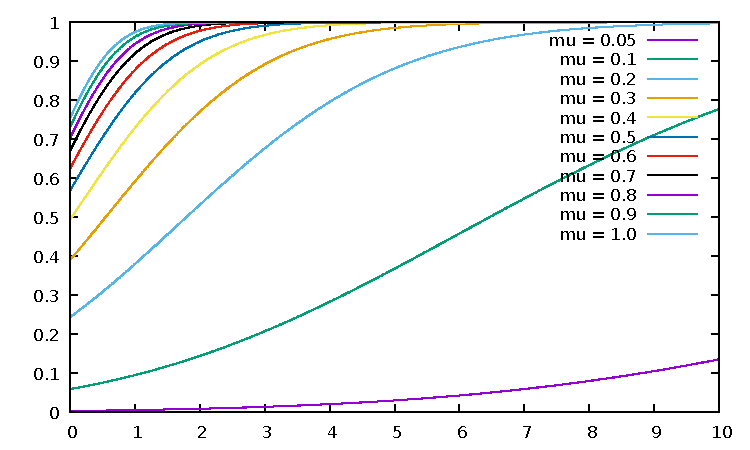
\includegraphics[width=1.00\linewidth]{small_mu.pdf}
        \caption{Shape of $J(r_{12};\mu)$ for small values of $\mu$.}
\end{figure*}
\begin{figure*}
 \label{fig_large_mu}
        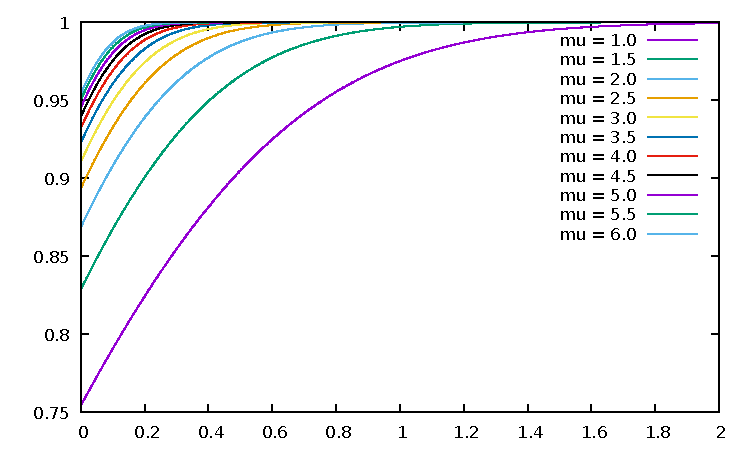
\includegraphics[width=1.00\linewidth]{large_mu.pdf}
        \caption{Shape of $J(r_{12};\mu)$ for large values of $\mu$.}
\end{figure*}
%%%%%%%%%%%%%%%%%%%%%%%%

\section{Technical stuffs: integration of the Jastrow factor}
\subsection{Fit of the Jastrow factor with usual functions}
\subsubsection{The fit of $f(r_{12},\mu)$}
We want to be able to fit $f(r_{12},\mu)$ with simple Slater and Gaussian type functions of the type 
\begin{equation}
 h(r_{12},\gamma,\delta) = e^{-\gamma r_{12} - \delta r_{12}^2}. 
\end{equation}
First we define the rescaled $\tilde{f}(r_{12},\mu)$ function as
\begin{equation}
 \begin{aligned}
 \tilde{f}(r_{12},\mu) & = f(r_{12},\mu)\times 2\sqrt{\pi}\mu  \\
                       & = \sqrt{\pi}\mu r_{12} \bigg( 1 - \text{erf}(\mu r_{12}) \bigg) - e^{-(\mu  r_{12})^2},
 \end{aligned}
\end{equation}
which has the advantage to take values in $[-1:0]$. 
The Taylor expansion of $\tilde{f}(r_{12},\mu)$ up to second order in $r_{12}$ is simply
\begin{equation}
 \tilde{f}(r_{12},\mu) = -1 + \sqrt{\pi}\mu r_{12} - \mu^2 (r_{12})^2 + o\big((r_{12})^2\big). 
\end{equation}
Then, we Taylor expand at second order the function $-h(r_{12},\gamma,\delta)$
\begin{equation}
 -h(r_{12},\gamma,\delta) = - 1 + \gamma r_{12} + \big( \delta - \frac{\gamma^2}{2} \big) (r_{12})^2.
\end{equation}
and the fit of $\tilde{f}(r_{12},\mu)$ by $h(r_{12},\gamma,\delta)$ is done by imposing the equality of the functions up to second order in $r_{12}$. 
This gives the following relationships
\begin{equation}
 \gamma(\mu) = \sqrt{\pi} \mu
\end{equation}
\begin{equation}
 \delta(\mu) = -\mu^2 + \frac{\gamma(\mu)^2}{2}.
\end{equation}
Therefore, we propose to fit the function $\tilde{f}(r_{12},\mu)$ by $h(r_{12},\gamma(\mu),\delta(\mu))$ 
\begin{equation}
 \label{fit_f_h}
  \tilde{f}(r_{12},\mu) = h(r_{12},\gamma,\delta) + O\big((r_{12})^2\big)
\end{equation}
As one can see from Fig. \ref{fit_small_mu} and \ref{fit_large_mu}, the agreement is pretty good between $\tilde{f}(r_{12},\mu)$ and $h(r_{12},\gamma,\delta)$, even for large values of $r_{12}$ and $\mu$. 
\begin{figure*}
 \label{fit_small_mu}
        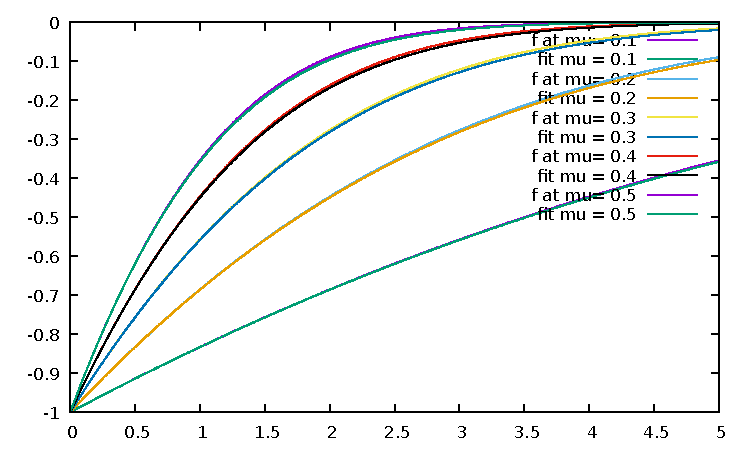
\includegraphics[width=1.00\linewidth]{fit_f_small.pdf}
        \caption{Fit of the function $\tilde{f}(r_{12},\mu)$ with the function $h(r_{12},\gamma(\mu),\delta(\mu))$, for small values of $\mu$. }
\end{figure*}
\begin{figure*}
 \label{fit_large_mu}
        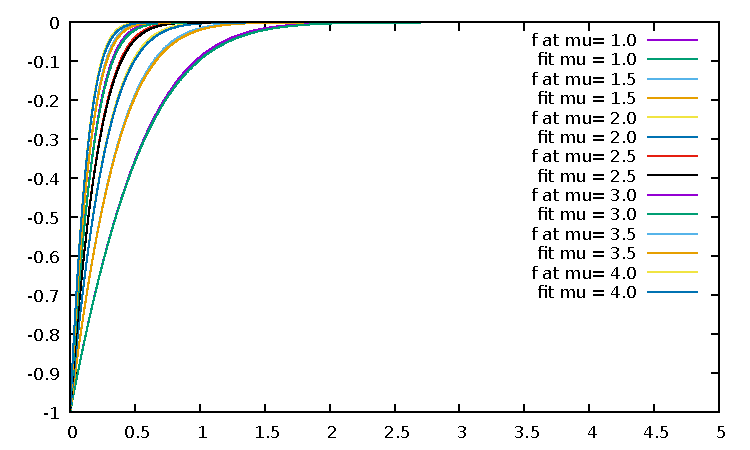
\includegraphics[width=1.00\linewidth]{fit_f_large.pdf}
        \caption{Fit of the function $\tilde{f}(r_{12},\mu)$ with the function $h(r_{12},\gamma(\mu),\delta(\mu))$, for large values of $\mu$. }
\end{figure*}

\subsubsection{Fit of the full Jastrow factor $J(r_{12},\mu)$}
Now we want to be able to represent the full Jastrow factor $J(r_{12},\mu)$ as a Taylor series of $\tilde{f}(r_{12},\mu)$. 
To do so we write
\begin{equation}
 \begin{aligned}
 \label{def_fit_j}
 J(r_{12},\mu) & = e^{f(r_{12},\mu)} \\
               & = e^{\frac{\tilde{f}(r_{12},\mu)}{2\sqrt{\pi}\mu}} \\
               & \approx e^{\frac{-h(r_{12},\gamma(\mu),\delta(\mu))}{2\sqrt{\pi}\mu}}. 
 \end{aligned}
\end{equation}
Then, as the function $-h(r_{12},\gamma(\mu),\delta(\mu)) \in [-1:0]$, we can Taylor expand the function $e^{-h(r_{12},\gamma(\mu),\delta(\mu))}$
\begin{equation}
 e^{-h(r_{12},\gamma(\mu),\delta(\mu))} = \sum_{n=0}^{\infty} \frac{1}{n!}\bigg(\frac{-h(r_{12},\gamma(\mu),\delta(\mu))}{2\sqrt{\pi}\mu}\bigg)^n. 
\end{equation}
By defining 
\begin{equation}
 a_n = \frac{1}{n!}\bigg(\frac{-1}{2\sqrt{\pi}\mu}\bigg)^n
\end{equation}
and because of the shape of the function $h(r_{12},\gamma,\delta)$ one obtains 
\begin{equation}
 \begin{aligned}
 \label{h_r_dl}
 e^{-h(r_{12},\gamma(\mu),\delta(\mu))} & = \sum_{n=0}^{\infty} a_n e^{-n\gamma(\mu)r_{12}} e^{-n\delta(\mu)(r_{12})^2} \\
                                      & = \sum_{n=0}^{\infty} a_n h\bigg( r_{12}, n\gamma(\mu),n\delta(\mu)\bigg).
 \end{aligned}
\end{equation}

\subsection{Important integrals with the Jastrow factor}
\subsubsection{Generic integrals}
We need two types of integrals. 
The first type are the normalization integrals 
\begin{equation}
 \label{def_big_sij}
 \mathcal{S}_{ij}^{kl}(\mu) = \int \int \dr{r_1}\dr{r_2} e^{f(r_{12},\mu)} \phi_i(\bd{r_1}) \phi_j(\bd{r_2}) \phi_k(\bd{r_1}) \phi_l(\bd{r_2})
\end{equation}
needed to normalize the wave function to unity or the pair density to the number of electron pairs. 
The second type of integrals are the interaction integrals 
\begin{equation}
 \label{def_big_vij}
 \mathcal{V}_{ij}^{kl}(\mu) = \int \int \dr{r_1}\dr{r_2} e^{f(r_{12},\mu)} \frac{\text{erf}(\mu r_{12})}{r_{12}}\phi_i(\bd{r_1}) \phi_j(\bd{r_2}) \phi_k(\bd{r_1}) \phi_l(\bd{r_2})
\end{equation}
needed to compute energy contributions.  

As computing analytical integrals of the type \eqref{def_big_sij} or \eqref{def_big_vij} is hard, we propose to compute analytical integrals of the type
\begin{equation}
 \label{def_s_ij}
 S_{jl}(\mu,\bd{r_1}) = \int \dr{r_2} e^{f(r_{12},\mu)} \phi_j(\bd{r_2}) \phi_l(\bd{r_2})
\end{equation}
and 
\begin{equation}
 \label{def_v_ij}
 V_{jl}(\mu,\bd{r_1}) = \int \dr{r_2} e^{f(r_{12},\mu)}\frac{\text{erf}(\mu r_{12})}{r_{12}}\phi_j(\bd{r_2}) \phi_l(\bd{r_2}).
\end{equation}
Therefore, we can compute $\mathcal{S}_{ij}^{kl}(\mu)$ and $\mathcal{V}_{ij}^{kl}(\mu)$ as
\begin{equation}
 \label{def_big_sij_bis}
 \mathcal{S}_{ij}^{kl}(\mu) = \int \dr{r_1} \phi_i(\bd{r_1})  \phi_k(\bd{r_1})S_{jl}(\mu,\bd{r_1})
\end{equation}
\begin{equation}
 \label{def_big_sij_bis}
 \mathcal{V}_{ij}^{kl}(\mu) = \int \dr{r_1} \phi_i(\bd{r_1})  \phi_k(\bd{r_1})V_{jl}(\mu,\bd{r_1})
\end{equation}
where the integration over $\bd{r_1}$ is performed using a regular DFT grid. 
The computation of \eqref{def_s_ij} and \eqref{def_v_ij} are not analytical in practice as the function $e^{f(r_{12},\mu)}$ might be hard to integrate. 
Nevertheless, as shown in Figs. \ref{fig_small_mu} and \ref{fig_large_mu},  and the function $\tilde{f}(r_{12},\mu)$ take values in $[-1:0]$, and therefore one can approximate the exponential by a Taylor development as in \eqref{def_fit_j}, and then use a Shank transformation to even gain in accuracy. 

\subsubsection{Basic framework to compute $S_{jl}(\mu,\bd{r_1})$ and $V_{jl}(\mu,\bd{r_1})$}
Assuming that the fit of of \eqref{def_fit_j} is valid, one can write $S_{jl}(\mu,\bd{r_1})$ as 
\begin{equation}
 \label{def_s_ij_dl_1} 
 \begin{aligned}
 S_{jl}(\mu,\bd{r_1})& = \int \dr{r_2} e^{f(r_{12},\mu)} \phi_j(\bd{r_2}) \phi_l(\bd{r_2}) \\
                     & =\int \dr{r_2} e^{\frac{-h(r_{12},\gamma(\mu),\delta(\mu))}{2\sqrt{\pi}\mu}}  \phi_j(\bd{r_2}) \phi_l(\bd{r_2}), 
 \end{aligned}
\end{equation}
which, according to \eqref{h_r_dl} becomes 
\begin{equation}
 \label{def_s_ij_dl_2} 
 \begin{aligned}
 S_{jl}(\mu,\bd{r_1})& = \int \dr{r_2} e^{f(r_{12},\mu)} \phi_j(\bd{r_2}) \phi_l(\bd{r_2}) \\
                     & =\int \dr{r_2} 
 \sum_{n=0}^{\infty} a_n h\big( r_{12}, n\gamma(\mu),n\delta(\mu)\big)
 \phi_j(\bd{r_2}) \phi_l(\bd{r_2}).
 \end{aligned}
\end{equation}
As in practice, we will truncate the sum in Eq. \eqref{def_s_ij_dl_2} up to some $N$ order, we can invert the discrete summation and integral. Therefore, we define the function $s_{ij}(\gamma,\delta)$ as 
\begin{equation} 
 \label{def_s_ij_atom}
 s_{jl}(\gamma,\delta,\bd{r_1}) = \int \dr{r_2} h( r_{12}, \gamma,\delta) \phi_j(\bd{r_2}) \phi_l(\bd{r_2}), 
\end{equation} 
and we write $S_{jl}(\mu,\bd{r_1})$ as 
\begin{equation}
 \label{def_s_ij_dl_3} 
 \begin{aligned}
 S_{jl}(\mu,\bd{r_1}) \approx & \sum_{n=0}^{N}  a_n 
                     & s_{ij}(n  \gamma(\mu),n  \delta(\mu),\bd{r_1}).
 \end{aligned}
\end{equation}
Here, the dependence in $\bd{r_1}$ of $S_{jl}(\mu,\bd{r_1})$ is within the function $h( r_{12}, \gamma,\delta)$ which can be written as a function of $\bd{r_2}$ depending on a vectorial parameter $\bd{r_1}$
\begin{equation}
 \begin{aligned}
  h( r_{12}, \gamma,\delta) = & h(\bd{r_1},\bd{r_2},\gamma,\delta) \\
                              & e^{-\gamma |\bd{r_1} - \bd{r_2}|} e^{-\delta |\bd{r_1} - \bd{r_2}|^2} 
 \end{aligned}
\end{equation}

Similarly, we can define the function 
\begin{equation} 
 \label{def_v_ij_atom}
 v_{jl}(\gamma,\delta,\mu,\bd{r_1}) = \int \dr{r_2} \frac{\text{erf}(\mu r_{12})}{r_{12}}h( r_{12}, \gamma,\delta) \phi_j(\bd{r_2}) \phi_l(\bd{r_2}), 
\end{equation}
and approximate the function $V_{jl}(\mu,\bd{r_1}) $ as
\begin{equation}
 \label{def_v_ij_dl}
 V_{jl}(\mu,\bd{r_1}) \approx \sum_{n=0}^{N}  a_n 
    v_{jl}(n  \gamma(\mu),n  \delta(\mu),\mu,\bd{r_1}).
\end{equation}

\subsubsection{Computation of $s_{ij}(\gamma,\delta,\bd{r_1})$ and $v_{ij}(\gamma,\delta,\mu,\bd{r_1})$}
The computation of $s_{ij}(\gamma,\delta,\bd{r_1})$ is \textit{a priori} not trivial as it contains a Slater function. 
Nevertheless, we can fit a Slater function with Gaussian functions (that is what quantum chemistry is about):
\begin{equation}
 e^{-X} = \sum_{m=1}^{N_s} c_m e^{-\zeta_m X^2}, 
\end{equation}
and, by posing $X=\gamma x$ one can fit any Slater function as
\begin{equation}
 e^{-\gamma x} = \sum_{m=1}^{N_s} c_m e^{-\zeta_m \gamma^2 x^2}. 
\end{equation}
To find the $\{c_m,\zeta_m\}$ parameters, I performed a Hartree Fock calculation on the Hydrogen atom using the $s$ functions of the ANO-RCC basis set which contains 8 gaussians.  
Therefore, computing $s_{jl}(\gamma,\delta,\bd{r_1})$ is nothing but a proper linear combination of Gaussian integrals. 

Of course, the same thing is valid for the computation of the $v_{ij}(\gamma,\delta,\mu,\bd{r_1})$. 

\section{Further thoughts ...}
Some stuffs to approximate maybe at second order ...
Higher order cusp condition
\begin{equation}
 \lim_{r_{12}\rightarrow 0}\deriv{\psiex}{r_{12}}{2} = \frac{1}{2} \deriv{\psiex}{r_{12}}{} = \frac{1}{4}\psiex(r_{12}=0)
\end{equation}
Now assume that $\psiex = e^{f}\phi$, then
\begin{equation}
 \deriv{e^{f}\phi }{r_{12}}{2} = \deriv{f}{r_{12}}{2} e^f \phi + \bigg(\deriv{f}{r_{12}}{} \bigg)^2 e^f\phi  
                               + \deriv{\phi}{r_{12}}{2}e^f
\end{equation}

\section{Derivation of Tew and applications to the Jastrow factor}
The present section provides some details about the very insightful derivations by Tew\cite{Tew-JCP-08} where the cusp conditions up to third order are proven. 
\subsection{The derivation by Tew}
Let us take a general Hamiltonian for $n$ particle within Coulomb interaction
\begin{equation}
 \bigg( -\sum_{i=1}^n \frac{\nabla_i^2}{m_i} + \sum_{i>j=1}^n \frac{Z_i Z_j}{r_{ij}}\bigg) \Psi = E \Psi .
\end{equation}
Here, the particles can be either protons and/or electrons, and therefore the wave function $\Psi$ depends on all coordinates \textit{i.e.} $\Psi(\bd{r}_1,\hdots,\bd{r}_n)$. 
Let us consider now the regions in configurational space where $0\le r_{12}\le\epsilon$ and $r_{i1},r_{i2}\gg \epsilon$ $(i>2)$, $r_{ij}\gg \epsilon$, $(i,j)>2$.

We transform the coordinate spaces from $\bd{r}_1$, $\bd{r}_2$ to $\br = \bd{r}_1 - \bd{r}_2$ and $\bs = (m_1 \bd{r}_1 + m_2 \bd{r}_2)/M$ with $M=m_1+m_2$. 
The derivative operator over $x_1$ becomes
\begin{equation}
 \begin{aligned}
 \deriv{}{x_1}{} = & \deriv{}{r_x}{} \deriv{r_x}{x_1}{} + \deriv{}{s_x}{} \deriv{s_x}{x_1}{} \\
                 = & \deriv{}{r_x}{} \deriv{x_1 - x_2}{x_1}{} + \deriv{}{s_x}{} \frac{1}{M}\deriv{m_1 x_1 + m_2 x_2}{x_1}{} \\
                 = & \deriv{}{r_x}{}                          + \deriv{}{s_x}{} \frac{m_1}{M}
 \end{aligned}
\end{equation}
and so
\begin{equation}
 \begin{aligned}
  \deriv{}{x_1}{2} = & \deriv{}{r_x}{2} + \bigg(\frac{m_1}{M} \bigg)^2 \deriv{}{s_x}{2} + 2\frac{m_1}{M}  \deriv{}{r_x}{}\deriv{}{s_x}{}.
 \end{aligned}
\end{equation}
Similarly, 
\begin{equation}
 \begin{aligned}
 \deriv{}{x_2}{} = - \deriv{}{r_x}{}    + \deriv{}{s_x}{} \frac{m_2}{M}
 \end{aligned}
\end{equation}
\begin{equation}
 \begin{aligned}
  \deriv{}{x_2}{2} = & \deriv{}{r_x}{2} + \bigg(\frac{m_2}{M} \bigg)^2 \deriv{}{s_x}{2} - 2\frac{m_2}{M}  \deriv{}{r_x}{}\deriv{}{s_x}{}.
 \end{aligned}
\end{equation}
Therefore, 
\begin{equation}
 \frac{1}{m_1} \deriv{}{x_1}{2}  + \frac{1}{m_2} \deriv{}{x_2}{2} = \frac{1}{M} \deriv{}{s_x}{2} + \frac{1}{\lambda} \deriv{}{r_x}{2}, 
\end{equation}
where $\lambda = m_1 m_2/M$.
Using the same change of variables for $(y_1,y_2)$ and $(z_1,z_2)$, the kinetic operator becomes then 
\begin{equation}
 \hat{T} = -\frac{\nabla^2_{\bs}}{2M} -\frac{\nabla^2_{\br}}{2\lambda} - \sum_{i=3}^n \frac{\nabla_i^2}{m_i}.
\end{equation}
In order to express the potential operator in terms of $\br$ and $\bs$, we introduce the cosines $\text{cos}(\theta_i)$ between the vectors $\bd{r}_{is} = \bd{r}_i - \bs$ and $\br$. 
To do so, we note that
\begin{equation}
 \begin{aligned}
 & \bd{r}_1 = \frac{m_2}{M}\br + \bs\\
 & \bd{r}_2 = \frac{m_1}{M}\br - \bs,
 \end{aligned}
\end{equation}
and 
\begin{equation}
 \begin{aligned}
 \bd{r}_{i1}& = \bd{r}_i - \bd{r}_1 = \bd{r}_i - \bd{s} - \frac{m_2}{M}\bd{r}\\
            & = \bd{r}_{is} - \frac{m_2}{M}\bd{r},
 \end{aligned}
\end{equation}
so 
\begin{equation}
 \begin{aligned}
 r_{i1}^2 &  = \bd{r_{i1}} \cdot \bd{r_{i1}} = r_{is}^2 + \bigg(\frac{m_2 r}{M}\bigg)^2 - 2\frac{m_2}{M} \bd{r}_{i1} \cdot \bd{r} \\
            & = r_{is}^2 + \bigg(\frac{m_2}{M}\bigg)^2 r^2 - 2\frac{m_2}{M} r_{is} r\, \text{cos}(\theta_i).
 \end{aligned}
\end{equation}
Similarly, we find for $r_{i2}^2$
\begin{equation}
 \begin{aligned}
 r_{i2}^2 &  = r_{is}^2 + \bigg(\frac{m_1}{M}\bigg)^2 r^2 + 2\frac{m_2}{M} r_{is} r\, \text{cos}(\theta_i).
 \end{aligned}
\end{equation}
In the region of interest, we can replace the potential in $1/r_{i1}$ by its partial wave expansion in terms of Legendre polynomials 
\begin{equation}
  \frac{1}{r_{i1}} = \frac{1}{r_{is}} \sum_{l=0}^\infty \bigg( \frac{m_2 r}{Mr_{is}} \bigg)^l P_l(\cos(\theta_i))
\end{equation}
which can be seen as a smart Taylor expansion of the annoying function $1/(1+X^2 -2 \alpha X)$. 
The same thing holds for $r_{i2}^{-1}$ by replacing $1$ by $2$ in the indices, and $\cos(\theta_i)$ by $-\cos(\theta_i)$. 
Therefore, the full Schroedinger equation becomes
\begin{equation}
 \begin{aligned}
  \bigg(&  -\frac{\nabla_{s}^2}{2 M}- \frac{\nabla_r^2}{2\lambda} - \sum_{i=3}^n \frac{\nabla_i^2}{m_i} + \frac{Z_1 Z_2}{r} 
   + \sum_{i>j=3}^n \frac{Z_i Z_j}{r_{ij}} \\
  &+ \sum_{i=3}^n \frac{Z_i}{r_{is}} \sum_{l=0}^\infty \bigg[Z_1 \bigg( \frac{m_2 r}{Mr_{is}}  \bigg)^l 
                                                            +Z_2 \bigg( -\frac{m_1 r}{Mr_{is}} \bigg)^l\bigg]P_l(\cos(\theta_i)) \bigg) \Psi = E \Psi.
 \end{aligned}
\end{equation}
We can then assign an order in $\epsilon$ to each term in the Hamiltonian, and we shall consider the terms of order 0 or less in $\epsilon$. 
Therefore, we have 
\begin{equation}
 \label{eq:schro_0}
 \bigg( - \frac{\nabla_r^2}{2\lambda} + \frac{Z_1 Z_2}{r} + \hat{S} + \mathcal{O}(\epsilon) \bigg) \Psi = E \Psi
\end{equation}
with the operator $\hat{S}$ being of zeroth order in $\epsilon$, which contains the kinetic energy of all particles except the inter particle kinetic term between 1 and 2, together with the zeroth order development of the Coulomb interaction minus that of particle 1 and 2
\begin{equation}
 \hat{S} = -\frac{\nabla_{s}^2}{2 M}  - \sum_{i=3}^n \frac{\nabla_i^2}{m_i}  + \sum_{i>j=3}^n \frac{Z_i Z_j}{r_{ij}} 
 + \sum_{i=3}^n \frac{Z_i}{r_{is}} \big( Z_1+Z_2 \big). 
\end{equation}
The terms in the Hamiltonian of order $\epsilon$ is 
\begin{equation}
 \mathcal{O}(\epsilon) = \sum_{i=3}^n \frac{Z_i}{r_{is}} \bigg[Z_1 \frac{m_2 r}{Mr_{is}}-Z_2 \frac{m_1 r}{Mr_{is}}\bigg],
\end{equation}
which vanishes for identical particles such as our dear electrons. 
The most general solution to Eq. \eqref{eq:schro_0} is given by 
\begin{equation}
 \label{eq:psi_gen}
 \Psi\big(\br,\bs \bd{r}_3, \hdots ,\bd{r}_n\big) = \sum_{l=0}^{\infty} \sum_{l=-m}^{+m} 
 r^l f_{lm}\big(r,\bs,\bd{r}_3, \hdots ,\bd{r}_n\big) Y_{lm}(\theta,\phi). 
\end{equation}
The differential operator $\nabla_r^2$ can be written in spherical coordinate as
\begin{equation}
 \begin{aligned}
 \nabla_r^2 f(r,\theta,\phi) = & \frac{1}{r} \deriv{}{r}{2} \bigg( r\,\, f(r,\theta,\phi) \bigg) \\
  &+ \frac{1}{r^2 \sin(\theta)}  \deriv{}{\theta}{} \bigg(\sin(\theta) \deriv{f(r,\theta,\phi)}{\theta}{} \bigg) \\
  &+ \frac{1}{r^2 \sin(\theta)}  \deriv{}{\phi}{2} f(r,\theta,\phi). 
 \end{aligned}
\end{equation}
Let us begin with $\frac{1}{r} \deriv{}{r}{2} \bigg( r\,\, \Psi(r,\theta,\phi,\hdots) \bigg)$.
First, $r\Psi(r,\theta,\phi,\hdots)$
\begin{equation}
 \Psi(r,\theta,\phi,\hdots) = \sum_{l=0}^{\infty} \sum_{l=-m}^{+m} r^{l+1}f_{lm}\big(r,\bs,\bd{r}_3, \hdots ,\bd{r}_n\big) Y_{lm}(\theta,\phi),
\end{equation}
and therefore, 
\begin{equation}
 \begin{aligned}
 \deriv{r\Psi}{r}{}  = & \sum_{l=0}^{\infty} \sum_{l=-m}^{+m}  Y_{lm}(\theta,\phi)\\  
  & \bigg[ (l+1) r^l f_{lm}\big(r,\bs,\bd{r}_3, \hdots \bd{r}_n\big) + r^{l+1} \deriv{}{r}{} f_{lm}\big(r,\bs,\bd{r}_3, \hdots \bd{r}_n\big)\bigg]. 
 \end{aligned}
\end{equation}
Then, 
\begin{equation}
 \begin{aligned}
 &\deriv{r\Psi}{r}{2}  = \sum_{l=0}^{\infty} \sum_{l=-m}^{+m}  Y_{lm}(\theta,\phi)\\   
 & \bigg[ l(l+1) r^{l-1} f_{lm}\big(r,\bs,\bd{r}_3, \hdots \bd{r}_n\big) + (l+1) r^l \deriv{}{r}{} f_{lm}\big(r,\bs,\bd{r}_3, \hdots \bd{r}_n\big) \\
+& (l+1) r^l  \deriv{}{r}{} f_{lm}\big(r,\bs,\bd{r}_3, \hdots \bd{r}_n\big) + r^{l+1} \deriv{}{r}{2} f_{lm}\big(r,\bs,\bd{r}_3, \hdots \bd{r}_n\big) \bigg],
 \end{aligned}
\end{equation}
and therefore 
\begin{equation}
 \label{eq:lapl}
 \begin{aligned}
 \frac{1}{r}\deriv{r\Psi}{r}{2}  =& \sum_{l=0}^{\infty} \sum_{l=-m}^{+m}  Y_{lm}(\theta,\phi) \, \, r^l\\
 & \bigg[  \deriv{}{r}{2} f_{lm}\big(r,\bs,\bd{r}_3, \hdots \bd{r}_n\big) 
 + \frac{2(l+1)}{r} \deriv{}{r}{} f_{lm}\big(r,\bs,\bd{r}_3, \hdots \bd{r}_n\big) \\
 & + \frac{l(l+1)}{r^2} f_{lm}\big(r,\bs,\bd{r}_3, \hdots \bd{r}_n\big) \bigg].
 \end{aligned}
\end{equation}
Unfortunatly, I don't find back the results of Eq. (16) of Ref. \onlinecite{Tew-JCP-08}, but this might be because the last term of equation \eqref{eq:lapl} involving $\frac{l(l+1)}{r^2}$ cancels out with the derivatives in $\theta$ and $\phi$. 
In any cases, we want to develop such an equation for $l=0$, which means that the last term in \eqref{eq:lapl} involving $\frac{l(l+1)}{r^2}$ vanishes, and that the part of the Laplacian involving angular derivatives vanishes also as $Y_0^0 = \frac{1}{\sqrt{4\pi}}$. 
Anyway, before taking the specific case of $l=0$, we will assume the result of Eq. (16) of Ref. \onlinecite{Tew-JCP-08}, which is  that the Schroedinger equation of \eqref{eq:schro_0} becomes
\begin{equation}
 \begin{aligned}
& \sum_{l=0}^\infty \sum_{m=-l}^{+l} r^l\bigg( \frac{1}{2\lambda} \bigg[ \deriv{}{r}{2} + \frac{2(l+1)}{r} \deriv{}{r}{}\bigg] \\ 
&- \frac{Z_1 Z_2}{r}  - \hat{S} + E \bigg) Y_{lm}(\theta,\phi) f_{lm}\big(r,\bs,\bd{r}_3, \hdots \bd{r}_n\big) =0.
 \end{aligned}
\end{equation}
Because of completeness and linear independence of the $Y_{lm}(\theta,\phi)$, this equation must stand for each value of $l,m$. Therefore, one obtains 
\begin{equation}
 \label{eq:schro_l}
 \begin{aligned}
& \bigg( \frac{1}{2\lambda} \bigg[ \deriv{}{r}{2} + \frac{2(l+1)}{r} \deriv{}{r}{}\bigg] 
&- \frac{Z_1 Z_2}{r}  - \hat{S} + E \bigg) f_{lm}\big(r,\bs,\bd{r}_3, \hdots \bd{r}_n\big) =0.
 \end{aligned}
\end{equation}
Now, we can Taylor expand up to some order $v$ the functions $f_{lm}\big(r,\bs,\bd{r}_3, \hdots \bd{r}_n\big) $ 
\begin{equation}
 \label{eq:tayl_flm}
 f_{lm}\big(r,\bs,\bd{r}_3, \hdots \bd{r}_n\big)  = \sum_{k=0}^v r^k f_{lm}^k\big(\bs,\bd{r}_3, \hdots \bd{r}_n\big), 
\end{equation}
and what has derived Tew in Ref. \onlinecite{Tew-JCP-08} is essentially the derivation of the three first terms $f_{lm}^k\big(\bs,\bd{r}_3, \hdots \bd{r}_n\big)$ for general $l$ and $k=0,1,2$. We will focus on $l=0$ for the rest of the section. 

\subsection{The case $l=0$}
From thereon, we focus on the part $l=0$ as it consists in two opposite spin electrons at coalescence. 
For the sake of compactness, we will use the following notations 
\begin{equation}
 f(\bd{R}) \equiv f\big(\bs,\bd{r}_3, \hdots \bd{r}_n\big)
\end{equation}
where $\bd{R}$ symbolises all other variables than $(r,\theta,\phi)$. 
Our goal is therefore to find the function $f_{00}\big(r,\bd{R})$,  which can be Taylor expanded as
\begin{equation}
 f_{00}\big(r,\bd{R}\big)  = \sum_{k=0}^v r^k f_{00}^k\big(\bd{R}\big). 
\end{equation}
Let us compute the action of the differential operator on $f_{00}\big(r,\bd{R}\big)$
\begin{equation}
 \begin{aligned}
 \frac{2}{r}\deriv{}{r}{} f_{00}\big(r,\bd{R}\big) = & \sum_{k=1}^v r^{k-2} 2 k\,f_{00}^k\big(\bd{R}\big)\\
 = & \frac{2}{r}f_{00}^1\big(\bd{R}\big) +  \sum_{k=2}^v r^{k-2} 2 k\,f_{00}^k\big(\bd{R}\big), 
 \end{aligned}
\end{equation}
\begin{equation}
 \deriv{}{r}{2} f_{00}\big(r,\bd{R}\big) = \sum_{k=2}r^{k-2} k(k-1) f_{00}^k\big(\bd{R}\big),
\end{equation}
which ads up to 
\begin{equation}
 \begin{aligned}
& \big( \deriv{}{r}{2} + \frac{2}{r}\deriv{}{r}{}  \big) f_{00}\big(r,\bd{R}\big) =  \frac{2}{r}f_{00}^1\big(\bd{R}\big) +
  \sum_{k=2}^v r^{k-2} (2 k + k(k-1)) f_{00}^k\big(\bd{R}\big). 
 \end{aligned}
\end{equation}
The potential operator acting on $f_{00}\big(r,\bd{R}\big)$ is simply
\begin{equation}
 \begin{aligned}
 \frac{Z_1 Z_2}{r} f_{00}\big(r,\bd{R}\big) = & \frac{Z_1 Z_2}{r} f_{00}^0\big(\bd{R}\big)+  & Z_1 Z_2 \sum_{k=1}^v r^{k-1} f_{00}^k\big(\bd{R}\big).  
 \end{aligned}
\end{equation}
We can then recompose the action of the Hamiltonian on the $l=0$ sector 
\begin{equation}
 \begin{aligned}
 \label{eq:power_exp}
&\frac{1}{\lambda r}f_{00}^1\big(\bd{R}\big) - \frac{Z_1 Z_2}{r} f_{00}^0\big(\bd{R}\big)
- Z_1 Z_2 \sum_{k=1}^v r^{k-1} f_{00}^k\big(\bd{R}\big) + \\ 
& \sum_{k=2}^v r^{k-2} (2 k + k(k-1)) f_{00}^k\big(\bd{R}\big) +
\big( E - \hat{S} \big) \sum_{k=0}^v r^k f_{00}^k\big(\bd{R}\big) = 0, 
 \end{aligned}
\end{equation}
and one can identify all terms having the same power of $r$. 
\subsection{The cusp conditions}
The term in $r^{-1}$ in \eqref{eq:power_exp} gives
\begin{equation}
 \frac{1}{\lambda} f_{00}^1\big(\bd{R}\big) - Z_1 Z_2 f_{00}^0\big(\bd{R}\big) = 0,
\end{equation}
or equivalently
\begin{equation}
 f_{00}^1\big(\bd{R}\big) = \lambda Z_1 Z_2 f_{00}^0\big(\bd{R}\big), 
\end{equation}
which for electrons, as $m_1 = m_2 = 1$ and $Z_1 = Z_2 = 1$, one obtains $ \lambda = \frac{1}{2}$, leading therefore to the famous cusp condition
\begin{equation}
 \label{eq:cusp_1}
 f_{00}^1\big(\bd{R}\big) = \frac{1}{2} f_{00}^0\big(\bd{R}\big). 
\end{equation}
The term in $r^0$ gives 
\begin{equation}
 \begin{aligned}
& -Z_1 Z_2 f_{00}^1\big(\bd{R}\big) + 6 f_{00}^2\big(\bd{R}\big) + \\
& \big( E - \hat{S} \big) f_{00}^0\big(\bd{R}\big) = 0, 
 \end{aligned}
\end{equation}
or equivalently
\begin{equation}
 \begin{aligned}
  6 f_{00}^2\big(\bd{R}\big) = Z_1 Z_2 f_{00}^1\big(\bd{R}\big) + \big( \hat{S} -E \big) f_{00}^0\big(\bd{R}\big)
 \end{aligned}
\end{equation}
which, thanks to Eq. \eqref{eq:cusp_1}, can be recast as 
\begin{equation}
 \begin{aligned}
 \label{eq:cusp_2}
  f_{00}^2\big(\bd{R}\big) = \frac{1}{6}\bigg( \lambda \big(Z_1 Z_2\big)^2  + \big( \hat{S} -E \big)\bigg) f_{00}^0\big(\bd{R}\big)
 \end{aligned}
\end{equation}
which coincides with the case $l=0$ of Eq. (20) of Ref. \onlinecite{Tew-JCP-08} which gives the second order derivative $f_{lm}^2\big(\bd{R}\big)$ for the general case $(l,m)$
\begin{equation}
 f_{00}^2\big(\bd{R}\big) = \frac{\lambda}{2l+3}\bigg( \frac{\lambda^2}{\lambda(l+1)} + \hat{S} -E \bigg) f_{00}^0\big(\bd{R}\big). 
\end{equation}

For electrons, $\lambda=1/2$ and therefore
\begin{equation}
 \label{eq:cusp_2_e}
f_{00}^2\big(\bd{R}\big) = \frac{1}{12} f_{00}^0\big(\bd{R}\big) + 
 \frac{1}{6} \big( \hat{S} -E \big) f_{00}^0\big(\bd{R}\big). 
\end{equation}

Eq. \eqref{eq:cusp_2_e} contains two type of contribution: the universal $\frac{1}{12} f_{00}^0\big(\bd{R}\big)$ contribution, and the system- and state-specific contribution of $\frac{1}{6} \big( \hat{S} -E \big) f_{00}^0\big(\bd{R}\big)$. 

\section{Using Tew's path for Jastrow factors}
\subsection{Position of the problem}
Let us assume now that the exact wave function can be written as 
\begin{equation}
 \label{eq:phi_j}
 \Psi\big(\br,\bd{R}\big) = e^{j(r)}\phi\big(\br,\bd{R}\big).
\end{equation}
As we impose that the correlation factor $j(r)$ only depends on $r$ (and not on $\theta$ or $\phi$), its expansion in terms of $Y_{lm}(\theta,\phi)$ is straightforward as it consists in the $l=0$ sector
\begin{equation}
 j(r) = r^0 j_{0}(r)Y_{00}(\theta,\phi).
\end{equation}
Nevertheless, the wave function $\phi\big(\br,\bd{R}\big)$ is expanded as in Eq. \eqref{eq:psi_gen}
\begin{equation} 
 \phi\big(\br,\bd{R}\big) = \sum_{l=0}^{\infty} \sum_{l=-m}^{+m} 
 r^l \phi_{lm}\big(r,\bd{R}\big) Y_{lm}(\theta,\phi), 
\end{equation}
Also, as $j(r) =$ coincides with the $l=0$ sector, so does $e^{j(r)}$, and therefore, focussing on the $l=0$ sector of Eq. \eqref{eq:schro_l},  we can write the Schroedinger equation for the wave function of type Eq. \eqref{eq:phi_j} 
\begin{equation}
 \label{eq:schro_phi_j}
 \begin{aligned}
& \bigg( \frac{1}{2\lambda} \bigg[ \deriv{}{r}{2} + \frac{2}{r} \deriv{}{r}{}\bigg] 
&- \frac{Z_1 Z_2}{r}  - \hat{S} + E \bigg) e^{j(r)}\phi_{00}\big(r,\bd{R}\big) =0.
 \end{aligned}
\end{equation}
Therefore, by identification with the $l=0$ sector of \eqref{eq:schro_l}, one can easily see that
\begin{equation}
 f_{00}\big(r,\bd{R}\big) = e^{j(r)}\phi_{00}\big(r,\bd{R}\big)
\end{equation}
as they solve the same partial differential equation. 
Therefore, we can identify term by term the cups conditions found by Tew and see how does it translate with the form of Eq. \eqref{eq:phi_j}. 

\subsection{Identifications term by term}
As in Eq. \eqref{eq:tayl_flm}, one can Taylor expand the functions $j(r)$ and $\phi_{00}\big(r,\bd{R}\big)$ in terms of powers of $r$
\begin{equation}
 \label{eq:tayl_phi00}
 \phi_{00}\big(r,\bd{R}\big)  = \sum_{k=0}^v r^k \phi_{00}^k\big(\bd{R}\big), 
\end{equation}
\begin{equation}
 \label{eq:tayl_j}
 j(r) = \sum_{k=0}^v r^k j^k.  
\end{equation}
As we are interested in the cusp condition up to second order, we will take $v=2$ and Taylor expand the function $e^j\phi$
\begin{equation}
 \label{eq:tayl_j_phi}
  e^{j(r)}\phi_{00}\big(r,\bd{R}\big) = e^{j^0 + j^1 r^1 + j^2 r^2}\bigg( \sum_{k=0}^2 r^k \phi_{00}^k\big(\bd{R}\big) \bigg). 
\end{equation}
With these notations, stopping the Taylor expansion at second order of Eq. \eqref{eq:tayl_j_phi} gives
\begin{equation}
 \begin{aligned}
 e^{j(r)}\phi_{00}\big(r,\bd{R}\big) = & e^{j^0}\bigg(\phi_0^0(\bd{R}) + r \big(\phi_0^0(\bd{R}) j^1 + \phi_0^1(\bd{R})\big) \\
 +& \frac{1}{2} r^2\big(\phi_0^0(\bd{R}) \big[ (j^1)^2 + 2j^2 \big] + 2 \phi_0^1(\bd{R}) j^1 + 2 \phi_0^2(\bd{R}) \big).  
 \end{aligned}
\end{equation}

Therefore, one can identify each terms
\begin{equation}
 \label{eq:f0_jphi}
 f_{00}^0(\bd{R}) = e^{j^0} \phi_0^0(\bd{R}),
\end{equation}
\begin{equation}
 \label{eq:f1_jphi}
 f_{00}^1(\bd{R}) = e^{j^0}\big(\phi_0^0(\bd{R}) j^1 + \phi_0^1(\bd{R})\big),
\end{equation}
\begin{equation}
 \label{eq:f2_jphi}
 f_{00}^2(\bd{R}) = e^{j^0}\frac{1}{2}\big(\phi_0^0(\bd{R}) \big[ (j^1)^2 + 2j^2 \big] + 2 \phi_0^1(\bd{R}) j^1 + 2 \phi_0^2(\bd{R}) \big).
\end{equation}

\subsubsection{Developing the first-order cusp condition}
Eq. \eqref{eq:f0_jphi} allows us to write the exact wave function at coalescence, and therefore one can rewrite the 
first order cusp condition of Eq. \eqref{eq:f1_jphi} as 
\begin{equation}
 \begin{aligned}
 f_{00}^1(\bd{R}) = & e^{j^0} \phi_0^0(\bd{R}) \bigg( j^1 + \frac{\phi_0^1(\bd{R})}{\phi_0^0(\bd{R})} \bigg) \\
                  = & f_{00}^0(\bd{R})         \bigg( j^1 + \frac{\phi_0^1(\bd{R})}{\phi_0^0(\bd{R})} \bigg) 
 \end{aligned}
\end{equation}
or equivalently
\begin{equation}
 \begin{aligned}
 \frac{f_{00}^1(\bd{R})}{f_{00}^0(\bd{R})} = j^1 + \frac{\phi_0^1(\bd{R})}{\phi_0^0(\bd{R})}. 
 \end{aligned}
\end{equation}
Therefore, if one assumes that the wave function $\phi_0(\br,\bd{R})$ is cusp-less, one finds 
\begin{equation}
 \begin{aligned}
  j^1 = \lambda Z_1 Z_2, 
 \end{aligned}
\end{equation}
which is equivalent to the usual cusp condition of Eq. \eqref{eq:cusp_1}. 

\subsubsection{Developing the second-order cusp condition}
The second order cusp condition of Eq. \eqref{eq:cusp_2} can be combined with Eq. \eqref{eq:f2_jphi} as 
\begin{equation}
  \begin{aligned}
& \frac{1}{6}\bigg( \lambda \big(Z_1 Z_2\big)^2  + \big( \hat{S} -E \big)\bigg) e^{j^0}\phi_0^0(\bd{R}) = \\
& e^{j^0}\frac{1}{2}\big(\phi_0^0(\bd{R}) \big[ (j^1)^2 + 2j^2 \big] + 2 \phi_0^1(\bd{R}) j^1 + 2 \phi_0^2(\bd{R}) \big),
  \end{aligned}
\end{equation}
which can be recombined as 
\begin{equation}
  \begin{aligned}
& \frac{1}{6}\lambda \big(Z_1 Z_2\big)^2 \phi_0^0(\bd{R}) - \frac{1}{2}\phi_0^0(\bd{R}) \big[ (j^1)^2 + 2j^2 \big] - \phi_0^1(\bd{R}) j^1  = \\
& \phi_0^2(\bd{R}) - \frac{1}{6}\big( \hat{S} -E \big) \phi_0^0(\bd{R}) ,
  \end{aligned}
\end{equation}
Note that if we set the jastrow factor to zero, we obtain 
\begin{equation}
  \begin{aligned}
 \phi_0^2(\bd{R}) =  \frac{1}{6}\lambda \big(Z_1 Z_2\big)^2 \phi_0^0(\bd{R}) + \frac{1}{6}\big( \hat{S} -E \big) \phi_0^0(\bd{R}),
  \end{aligned}
\end{equation}
which is equivalent to Eq. \eqref{eq:cusp_2_e}. 


Now let us assume that $\phi_0^1(\bd{R}) = 0$ and that $j^1 = \lambda Z_1 Z_2$, 
\begin{equation}
  \begin{aligned}
& \phi_0^0(\bd{R}) \bigg( \lambda \big(Z_1 Z_2\big)^2 \big( \frac{1}{6} - \frac{1}{2} \lambda\big) - j^2 \bigg) = \\
& \phi_0^2(\bd{R}) - \frac{1}{6}\big( \hat{S} -E \big) \phi_0^0(\bd{R}) ,
  \end{aligned}
\end{equation}
or equivalently
\begin{equation}
  \begin{aligned}
& \lambda \big(Z_1 Z_2\big)^2 \big( \frac{1}{6} - \frac{1}{2} \lambda\big) - j^2  = \\
& \frac{1}{\phi_0^0(\bd{R})} \bigg( \phi_0^2(\bd{R}) - \frac{1}{6}\big( \hat{S} -E \big) \phi_0^0(\bd{R}) \bigg) ,
  \end{aligned}
\end{equation}
with $Z_1 = Z_2 = 1$, $\lambda = \frac{1}{2}$ 
\begin{equation}
  \begin{aligned}
& \frac{1}{2}\big( \frac{1}{6} - \frac{1}{4} \big) - j^2  = \\
& \frac{1}{\phi_0^0(\bd{R})} \bigg( \phi_0^2(\bd{R}) - \frac{1}{6}\big( \hat{S} -E \big) \phi_0^0(\bd{R}) \bigg) ,
  \end{aligned}
\end{equation}
\begin{equation}
 \label{eq:j2}
  \begin{aligned}
& -\frac{1}{24} - j^2  = \\
& \frac{1}{\phi_0^0(\bd{R})} \bigg( \phi_0^2(\bd{R}) - \frac{1}{6}\big( \hat{S} -E \big) \phi_0^0(\bd{R}) \bigg) .
  \end{aligned}
\end{equation}
An important point of Eq. \eqref{eq:j2}, is that the left part is independent of $\bd{R}$ whereas the right hand side is dependent on $\bd{R}$. Therefore, one must have
\begin{equation}
 \label{eq:univ}
 \phi_0^2(\bd{R}) - \frac{1}{6}\big( \hat{S} -E \big) \phi_0^0(\bd{R}) = 0, 
\end{equation}
or 
\begin{equation}
 \label{eq:phi02}
 \phi_0^2(\bd{R}) = \frac{1}{6}\big( \hat{S} -E \big) \phi_0^0(\bd{R}), 
\end{equation}
but Eq. \eqref{eq:univ} also implies that 
\begin{equation}
 \label{eq:j02}
 j^2 = -\frac{1}{24},
\end{equation}
which coincides with the result of Tew in Ref. \onlinecite{Tew-JCP-08} regarding the minimal Jastrow factor on-top of a HF wave function. 

The Eqs. \eqref{eq:phi02} and \eqref{eq:j02} suggest two important things: if one uses a cusp-less wave function of type $\phi_0(\bd{r},\bd{R})$ multiplied by a general Jastrow factor $j(r)$ only depending on the inter-electronic distance $r$, then the analysis up to zeroth-order in $r$ provides you the first and second order derivatives of the Jastrow factor which are $1/2$ and $-1/24$. 
The Eq. \eqref{eq:phi02} also tells you that, provided that you take the Jastrow factor with the correct first and second derivatives, then the second order in a given configurational point $\bd{R}$ obeys a mean-field equation like. 


\subsection{Eigenequation for $\phi$: the similarity transformed Hamiltonian}
\subsubsection{Expression of the similarity transformed Hamiltonian}
Another way to see the problem is to multiply Eq. \eqref{eq:schro_phi_j} by $e^{-j(r)}$ to obtain a similarity transformed or trans-correlated Hamiltonian
\begin{equation}
 \label{eq:schro_tilde_phi_j}
 \begin{aligned}
 e^{-j(r)} \bigg( \frac{1}{2\lambda} \bigg[ \deriv{}{r}{2} + \frac{2}{r} \deriv{}{r}{}\bigg] - \frac{Z_1 Z_2}{r}  - \hat{S} + E \bigg) e^{j(r)}\phi_{00}\big(r,\bd{R}\big) =0, 
 \end{aligned}
\end{equation}
which can be written as 
\begin{equation}
 \label{eq:htilde_phi}
 \bigg(E -\tilde{\mathcal{H}}[j]\bigg) \phi_{00}\big(r,\bd{R}\big) = 0,
\end{equation}
with the similarity transformed Hamiltonian $ \tilde{\mathcal{H}}[j] $ defined by
\begin{equation}
  \tilde{\mathcal{H}}[j]  = e^{-j(r)} \bigg( -\frac{1}{2\lambda} \bigg[ \deriv{}{r}{2} + \frac{2}{r} \deriv{}{r}{}\bigg] 
+ \frac{Z_1 Z_2}{r}  + \hat{S}  \bigg) e^{j(r)}.
\end{equation}

An important consequence of the choice of $f(r)$ (which only depends on $r$), is that the operator $\hat{S}$, which depends on all variables but $r,\theta,\phi$, leaves $f(r)$ untouched, \textit{i.e.}
\begin{equation}
 \hat{S} f(r) = f(r).
\end{equation}
Therefore, the similarity transformed Hamiltonian can be written as
\begin{equation}
  \tilde{\mathcal{H}}[j]  =  -\frac{1}{2\lambda} e^{-j(r)} \bigg[ \deriv{}{r}{2} + \frac{2}{r} \deriv{}{r}{}\bigg]  e^{j(r)}
+ \frac{Z_1 Z_2}{r}  + \hat{S},
\end{equation}
and Eq. \eqref{eq:schro_tilde_phi_j} can be written as
\begin{equation}
 \frac{1}{2\lambda} e^{-j(r)} \bigg[ \deriv{}{r}{2} + \frac{2}{r} \deriv{}{r}{}\bigg]  e^{j(r)}\phi_{00}(r,\bd{R}) 
- \bigg( \frac{Z_1 Z_2}{r}  + \hat{S} -E \bigg) \phi_{00}(r,\bd{R}) = 0.
\end{equation}
Doing the math one obtains that 
\begin{equation}
 e^{-j(r)} \frac{2}{r} \deriv{}{r}{} e^{j(r)} \cdot = \frac{2}{r}\bigg( \deriv{}{r}{} + \deriv{j}{r}{} \bigg),
\end{equation}
\begin{equation}
 e^{-j(r)} \deriv{}{r}{2} e^{j(r)} \cdot = \deriv{j}{r}{2} + \bigg( \deriv{j}{r}{} \bigg)^2 + 2 \deriv{j}{r}{} \deriv{}{r}{} + \deriv{}{r}{2},
\end{equation}
and therefore the action on a given $\phi(r)$ of the similarity transformed kinetic operator can be written as 
\begin{equation}
 \begin{aligned}
  e^{-j(r)} \bigg[ \deriv{}{r}{2} + &\frac{2}{r} \deriv{}{r}{}\bigg]  e^{j(r)} \phi(r) =  \deriv{\phi}{r}{2} + \frac{2}{r} \bigg( \deriv{\phi}{r}{}+ \deriv{j}{r}{}\phi(r) \bigg) \\ 
& + 2 \deriv{j}{r}{} \deriv{\phi}{r}{} + \bigg[\deriv{j}{r}{2} + \bigg( \deriv{j}{r}{} \bigg)^2\bigg] \phi(r). 
 \end{aligned}
\end{equation}
Therefore, one can recombine the right hand side of Eq. \eqref{eq:htilde_phi} in 
\begin{equation}
 \label{eq:tilde_2}
 \begin{aligned}
  \bigg(E -\tilde{\mathcal{H}}[j]\bigg) \phi_{00}\big(r,\bd{R}\big) = & \frac{1}{2\lambda} \bigg( \deriv{\phi_{00}\big(r,\bd{R}\big)}{r}{2} +   \deriv{\phi_{00}\big(r,\bd{R}\big)}{r}{} \bigg[ \frac{2}{r}+ 2 \deriv{j(r)}{r}{}\bigg] \bigg)  \\
& - \frac{1}{r} \bigg( Z_1 Z_2 - \frac{1}{\lambda}  \deriv{j(r)}{r}{} \bigg) \phi_{00}\big(r,\bd{R}\big) \\
& + \bigg( \frac{1}{2\lambda}\bigg[ \deriv{j(r)}{r}{2} + \bigg(\deriv{j(r)}{r}{}\bigg)^2\bigg] + E  - \hat{S} \bigg)\phi_{00}\big(r,\bd{R}\big).
 \end{aligned}
\end{equation}
Therefore, one can write an explicit form of $\tilde{\mathcal{H}}[j]$ as 
\begin{equation}
 \label{def:htilde}
 \begin{aligned}
 \tilde{\mathcal{H}}[j] = & - \frac{1}{2\lambda} \bigg( \deriv{}{r}{2} + \bigg[ \frac{2}{r}+  2 \deriv{j(r)}{r}{}\bigg] \deriv{}{r}{} \bigg) \\
 & + \frac{1}{r} \bigg( Z_1 Z_2 - \frac{1}{\lambda}  \deriv{j(r)}{r}{} \bigg) \\
 &- \bigg( \frac{1}{2\lambda}\bigg[ \deriv{j(r)}{r}{2} + \bigg(\deriv{j(r)}{r}{}\bigg)^2\bigg] - \hat{S} \bigg). 
 \end{aligned}
\end{equation}

\subsubsection{Taylor expansion of $\tilde{\mathcal{H}}[j]$}
By introducing the Taylor expansion of the function $j(r)$, one obtains 
\begin{equation}
 \label{eq:sim_h}
 \begin{aligned}
 e^{-j(r)} \bigg[ \deriv{}{r}{2} + & \frac{2}{r} \deriv{}{r}{}\bigg]  e^{j(r)} \phi(r) = \deriv{\phi}{r}{2} + \frac{2}{r}\bigg( \deriv{\phi}{r}{} + \phi(r)\sum_{k=1}^v k\, r^{k-1} j^k \bigg) \\
 + & 2 \bigg( \sum_{k=1}^v k \, r^{k-1} j^k  \bigg) \deriv{\phi}{r}{} \\
 + & \bigg(\sum_{k=2}^v k(k-1) r^{k-2} j^k + \sum_{k=1}^v\sum_{n=1}^v n \, k \, r^{k+n-2} j^k j^n\bigg)\phi(r) \, .
 \end{aligned}
\end{equation}
As proposed by Tew in Eq. \eqref{eq:schro_0}, we only keep the terms of order smaller or equal to zero in $r$. 
Therefore, sorting by importance in terms of $r$ and stopping at $r^0$, equation Eq. \eqref{eq:sim_h} becomes
\begin{equation}
 \label{eq:sim_kin_1}
 \begin{aligned}
 e^{-j(r)} \bigg[ \deriv{}{r}{2} + & \frac{2}{r} \deriv{}{r}{}\bigg]  e^{j(r)} \phi(r) =  r^{-1} 2 \bigg( \deriv{\phi}{r}{} + j^1 \phi(r)\bigg)\\
& + r^0 \bigg( \deriv{\phi}{r}{2} + 2 j^1 \deriv{\phi}{r}{} + \bigg[  6 j^2  + \big(j^1\big)^2\bigg] \phi(r) \bigg) \, .
 \end{aligned}
\end{equation}
which, by dividing by $2\lambda$ gives
\begin{equation}
 \label{eq:sim_kin_2}
 \begin{aligned}
 \frac{1}{2\lambda}e^{-j(r)} \bigg[ \deriv{}{r}{2} + & \frac{2}{r} \deriv{}{r}{}\bigg]  e^{j(r)} \phi(r) =  r^{-1} \frac{1}{\lambda}\bigg( \deriv{\phi}{r}{} + j^1 \phi(r)\bigg)\\
& + r^0 \frac{1}{\lambda}\bigg( \frac{1}{2}\deriv{\phi}{r}{2} + j^1 \deriv{\phi}{r}{} + \bigg[  3 j^2  + \frac{\big(j^1\big)^2}{2}\bigg] \phi(r) \bigg) \, .
 \end{aligned}
\end{equation}
Then, one can compute the action of the pure potential part of $\tilde{\mathcal{H}}[f]$ 
\begin{equation}
 \label{eq:pot}
 \begin{aligned}
& - \frac{1}{\lambda}\bigg( \frac{\lambda Z_1 Z_2}{r}  + \lambda\big(\hat{S} -E\big) \bigg) \phi_{00}(r,\bd{R})  
 \end{aligned}
\end{equation}
Eventually, one can recombine Eqs. \eqref{eq:pot} and \eqref{eq:sim_kin} 
\begin{equation}
 \label{eq:sim_tot}
 \begin{aligned}
& r^{-1} \frac{1}{\lambda}\bigg( \deriv{\phi_{00}(r,\bd{R})}{r}{} + \bigg[j^1-\lambda Z_1 Z_2\bigg]\phi_{00}(r,\bd{R})\bigg)  \\
& + r^0 \frac{1}{\lambda} \bigg( \frac{1}{2}\deriv{\phi_{00}(r,\bd{R})}{r}{2} + j^1 \deriv{\phi_{00}(r,\bd{R})}{r}{}\bigg) \\
& + r^0 \frac{1}{\lambda} \bigg( j^2  + \frac{\big(j^1\big)^2}{2} + \lambda \big( E - \hat{S} \big) \bigg) \phi_{00}(r,\bd{R}) = 0.
 \end{aligned}
\end{equation}
Before determining the cusp conditions, let us discuss some clues about the validity domain of Eq. \eqref{eq:sim_tot}. 
Eq. \eqref{eq:sim_tot} must hold for all  $\bd{R}$ and $r$ such that $r\ll r_{is},\,i=3,n $, which means when two electrons are well isolated from the rest of the other particles. 

\subsubsection{Cusp conditions}
We are going now to focus on the cusp conditions with the similarity transformed Hamiltonian. 
Starting from Eq. \eqref{eq:sim_tot}, one can introduce the Taylor expansion of Eq. \eqref{eq:tayl_phi00} and identify the terms in $r^{-1}$, which gives 
\begin{equation}
 \begin{aligned}
  \phi_{00}^1(\bd{R}) +  \bigg( j^1 - \lambda Z_1 Z_2\bigg) \phi_{00}^0(\bd{R}) = 0, 
 \end{aligned}
\end{equation}
which is nothing but
\begin{equation}
 \phi_{00}^1(\bd{R}) = \phi_{00}^0(\bd{R}) \bigg( \lambda Z_1 Z_2 - j^1\bigg). 
\end{equation}
Therefore, if we impose that $j(r)$ has the correct cusp (\textit{i.e.} $j^1 = Z_1 Z_2 \lambda$) then one obtains 
\begin{equation}
 \phi_{00}^{1}(\bd{R}) = 0, 
\end{equation}
which means that the wave function $\phi_{00}(r,\bd{R})$ is cusp-less. The other way around is also true: if we impose that the wave function $\phi_{00}(r,\bd{R})$ is cusp-less, then the Jastrow factor must recover the cusp. 
Also, if we set the jastrow factor to zero, then one obtains the usual cusp condition, \textit{i.e.} $\phi_{00}^1(\bd{R}) = \lambda Z_1 Z_2 \phi_{00}^0(\bd{R}) $.

We can do the same thing and look at all terms of order $0$ in $r$, 
\begin{equation}
 \begin{aligned}
& 3 \phi_{00}^2(\bd{R}) + 2 j^1 \phi_{00}^1(\bd{R}) -\lambda Z_1 Z_2 \phi^1_{00}(\bd{R}) \\
+& \big( j^2 + \frac{\big(j^1\big)^2}{2}\big)\phi_{00}^0(\bd{R}) + \lambda\big( E - \hat{S} \big)\phi_{00}^0(\bd{R}) = 0. 
 \end{aligned}
\end{equation}
or 
\begin{equation}
 \phi_{00}^2(\bd{R}) = \frac{\lambda}{3}\bigg( \phi_{00}^1(\bd{R}) \big(  Z_1 Z_2 - 2 \frac{j^1}{\lambda} \big) + \phi_{00}^0(\bd{R}) \bigg[ \hat{S} - E - \frac{1}{\lambda}\bigg( j^2 + \frac{\big(j^1\big)^2}{2}\bigg) \bigg] \bigg).
\end{equation}

If we set $j(r)=0$, we  find 
\begin{equation}
 \phi_{00}^2(\bd{R}) = \frac{\lambda}{3} \bigg( Z_1 Z_2 \phi^1_{00}(\bd{R}) + \big( \hat{S} - E\big)\phi_{00}^0(\bd{R}) \bigg) = 0.
\end{equation}
By using the first-order cusp condition, one finds 
\begin{equation}
 \phi_{00}^2(\bd{R}) = \frac{\lambda}{3} \bigg( \lambda (Z_1 Z_2)^2 \phi^0_{00}(\bd{R}) + \big( \hat{S} - E\big)\phi_{00}^0(\bd{R}) \bigg) = 0.
\end{equation}
which corresponds to the original second-order cusp condition. 

\subsection{Analysis of a Hamiltonian with a long-range interaction}
\subsubsection{The main equations}
Let us now take the case of an Hamiltonian with a long-range interaction $\text{erf}(\mu r)/r$ as those used in RS-DFT. 
The effective Schroedinger equation is then 
\begin{equation}
 \begin{aligned}
& \tilde{H}^\mu \Phi^{\mu} = \tilde{E} \Phi^{\mu} \Leftrightarrow \\
& \bigg( -\sum_{i=1}^n \frac{\nabla_i^2}{m_i} + \sum_{i=1}^n v_{\text{Hxc}}(\bd{r}_i) + \sum_{i>j=1}^n Z_i Z_j \frac{\text{erf}(\mu r_{ij})}{r_{ij}}\bigg) \Phi^{\mu} = \tilde{E} \Phi^{\mu}
 \end{aligned}
\end{equation}
where $v_{\text{Hxc}}(\bd{r})$ is the short-range potential maintaining the exact density, \textit{i.e.} $n_{\Phi_{\mu}} = n_{\Psi}$, and $\tilde{E}$ is the effective eigenvalue equation which is not physical. 
Following the path of Tew, we Taylor expand the effective Hamiltonian in term of $r$ and keep the term of order inferior or equal to zero. 
%The long-range interaction becomes
%\begin{equation}
% \frac{\text{erf}(\mu_{ij})}{r_{ij}} = \frac{2 \mu}{\sqrt{\pi}},
%\end{equation}
The effective potentials $v_{\text{Hxc}}(\bd{r}_i)$ for $i=1,2$ become 
\begin{equation}
 v_{\text{Hxc}}(\bd{r}_1) = v_{\text{Hxc}}(\bs) + \nabla_{\bd{r}} v_{\text{Hxc}}(\frac{m_2}{M}\br + \bs) \bigg|_{\br = {\bd{0}}} \cdot \text{d}\br
\end{equation}
\begin{equation}
 v_{\text{Hxc}}(\bd{r}_2) = v_{\text{Hxc}}(-\bs) + \nabla_{\bd{r}} v_{\text{Hxc}}(\frac{m_1}{M}\br - \bs) \bigg|_{\br = {\bd{0}}}  \cdot \text{d}\br 
\end{equation}
The terms involving the gradients with respect to $\bd{r}$ are necessary of order 1 in $r$ and therefore can be ignored. 
We end up with the following effective Hamiltonian $\tilde{H}^\mu $ at order lower or equal to 0 in $r$ 
\begin{equation}
 \label{eq:hmu}
 \bigg( - \frac{\nabla_r^2}{2\lambda} + Z_1 Z_2\frac{\text{erf}(\mu r)}{r} + \hat{S}^\mu + \mathcal{O}(\epsilon) \bigg) \Phi^{\mu} = \tilde{E} \Phi^\mu
\end{equation}
with the effective operator $\hat{S}^\mu$ being
\begin{equation}
 \begin{aligned}
 \hat{S}^\mu = &-\frac{\nabla_{s}^2}{2 M}  - \sum_{i=3}^n \frac{\nabla_i^2}{m_i}  + \sum_{i>j=3}^n Z_i Z_j\frac{\text{erf}(\mu r_{ij})}{r_{ij}}  \\ 
& + \sum_{i=3}^n Z_i\frac{\text{erf}(\mu r_{is})}{r_{is}} \big( Z_1+Z_2 \big) \\ 
&+ v_{\text{Hxc}}(\bs) + v_{\text{Hxc}}(-\bs) + \sum_{i=3}^n v_{\text{Hxc}}(\bd{r}_i). 
 \end{aligned}
\end{equation}
We can then do the same analysis as before, which is expand the wave function $\Phi^{\mu}$ in spherical harmonics 
\begin{equation}
 \Phi^{\mu}(\br,\bd{R}) = \sum_{l=0}^\infty r^l \sum_{m=-l}^{+l} \Phi_{lm}^{\mu}(r,\bd{R})Y_{lm}(\theta,\phi), 
\end{equation}
then inject in the Schroedinger-like equation Eq. \eqref{eq:hmu}, and then focus on the $l=0$ sector, which gives
\begin{equation}
 \begin{aligned}
 \label{eq:hmu_2}
 \bigg( \frac{1}{2\lambda} \bigg[ \deriv{}{r}{2} + \frac{2}{r} \deriv{}{r}{}\bigg] & - Z_1 Z_2 \frac{\text{erf}(\mu r)}{r}
- \hat{S}^\mu + \tilde{E} \bigg) \Phi_{00}^{\mu}\big(r,\bd{R}\big) = 0. 
 \end{aligned}
\end{equation}


\subsubsection{The cusp conditions}
One can then Taylor expand in powers of $r$ the solution $\Phi_{00}^{\mu}\big(r,\bd{R}\big)$ 
\begin{equation}
 \Phi_{00}^{\mu}\big(r,\bd{R}\big) = \sum_{k=0}^v r^k \Phi_{00}^{k,\mu}\big(\bd{R}\big),
\end{equation}
and then plug into Eq. \eqref{eq:hmu_2}, which, according the Taylor development of $\text{erf}(\mu r)/r$ gives
\begin{equation}
 \begin{aligned}
 r^{-1} \frac{1}{\lambda} & \sum_{k=1}^v k r^{k-1} \Phi_{00}^{k,\mu}\big(\bd{R}\big) + \frac{1}{2\lambda} \sum_{k=2}^v r^{k-2} k(k-1) \Phi_{00}^{k,\mu}\big(\bd{R}\big)\\ 
& + \bigg( - Z_1 Z_2 \frac{2 \mu}{\sqrt{\pi}}  - \hat{S}^\mu + \tilde{E} \bigg)  \sum_{k=0}^v r^k \Phi_{00}^{k,\mu}\big(\bd{R}\big) = 0.
 \end{aligned}
\end{equation}
The identification for $r^{-1}$ gives
\begin{equation}
 \frac{1}{\lambda} \Phi_{00}^{1,\mu}\big(\bd{R}\big) = 0
\end{equation}
which says that the wave function $\Phi_{00}^{\mu}\big(r,\bd{R}\big)$ has no cusp. 

Then, the terms in $r^0$ are 
\begin{equation}
 \frac{1}{\lambda}2 \Phi_{00}^{2,\mu}\big(\bd{R}\big) + \frac{1}{2 \lambda} 2 \Phi_{00}^{2,\mu}\big(\bd{R}\big) 
 + \bigg( - Z_1 Z_2 \frac{2 \mu}{\sqrt{\pi}} - \hat{S}^\mu + \tilde{E}   \bigg) \Phi_{00}^{0,\mu}\big(\bd{R}\big) = 0,
\end{equation}
which translates into 
\begin{equation}
 \Phi_{00}^{2,\mu}\big(\bd{R}\big) = \frac{\lambda}{3}\bigg( Z_1 Z_2 \frac{2 \mu}{\sqrt{\pi}} + \hat{S}^\mu - E\bigg) \Phi_{00}^{0,\mu}\big(\bd{R}\big). 
\end{equation}
Therefore, the second-order derivative in $r$ depends on $\mu$ but also on $\bd{R}$. 

\subsubsection{Linking RS-DFT and jastrows}
We wan to make a mapping between the effective trans-correlated Hamiltonian $\tilde{\mathcal{H}}[j]$ of Eq. \eqref{def:htilde} and that of $\tilde{H}^\mu$ of Eq. \eqref{eq:hmu_2}. 
More precisely, we want to find the conditions on $j(r)$ such that the eigenfunction $\Phi_{00}\big(r,\bd{R}\big)$ of $\tilde{\mathcal{H}}[j]$ coincide with the eigenfunction $\Phi_{00}^{\mu}\big(r,\bd{R}\big)$ of $\tilde{H}^\mu$. 
Let us rewrite the two equations 
\begin{equation}
 \label{def:htilde2}
 \begin{aligned}
& \bigg(\tilde{\mathcal{H}}[j] - E \bigg) \Phi_{00}\big(r,\bd{R}\big) = 0 \Leftrightarrow \\ 
& - \frac{1}{2\lambda} \bigg( \deriv{}{r}{2}\Phi_{00}\big(r,\bd{R}\big) + \bigg[ \frac{2}{r}+  2 \deriv{j(r)}{r}{}\bigg] \deriv{}{r}{}\Phi_{00}\big(r,\bd{R}\big) \bigg) \\
 & + \frac{1}{r} \bigg( Z_1 Z_2 - \frac{1}{\lambda}  \deriv{j(r)}{r}{} \bigg) \Phi_{00}\big(r,\bd{R}\big) \\
 & - \frac{1}{2\lambda}\bigg[ \deriv{j(r)}{r}{2} + \bigg(\deriv{j(r)}{r}{}\bigg)^2\bigg]\Phi_{00}\big(r,\bd{R}\big)  \\ 
& + \big( \hat{S} - E\big) \Phi_{00}\big(r,\bd{R}\big) = 0, 
 \end{aligned}
\end{equation}
and 
\begin{equation}
 \begin{aligned}
 \label{eq:hmu_3}
& \bigg( \tilde{H}^\mu - \tilde{E} \bigg) \Phi_{00}^{\mu}\big(r,\bd{R}\big) = 0 \Leftrightarrow\\
& -\frac{1}{2\lambda} \bigg[ \deriv{}{r}{2} \Phi_{00}^{\mu}\big(r,\bd{R}\big) + \frac{2}{r} \deriv{}{r}{}\Phi_{00}^{\mu}\big(r,\bd{R}\big) \bigg] \\ 
& + Z_1 Z_2 \frac{\text{erf}(\mu r)}{r}\Phi_{00}^{\mu}\big(r,\bd{R}\big) \\
&+ \big(\hat{S}^\mu - \tilde{E}\big) \Phi_{00}^{\mu}\big(r,\bd{R}\big) = 0. 
 \end{aligned}
\end{equation}
In Eq. \eqref{eq:hmu_3} and \eqref{def:htilde2} there are two types of terms: the universal terms only depending in $r$ and the terms depending on the wave function and the coordinates of the other electrons $\bd{R}$.  
We want to make a mapping only in terms of the universal terms, and therefore we propose the following statement 
\begin{equation}
 \big(\hat{S}^\mu - \tilde{E}\big) \Phi_{00}^{\mu}\big(r,\bd{R}\big) = \big( \hat{S} - E\big) \Phi_{00}\big(r,\bd{R}\big) - \frac{1}{\lambda} \deriv{j(r)}{r}{} \Phi_{00}\big(r,\bd{R}\big). 
\end{equation}

Under that assumption, the match between Eq. \eqref{eq:hmu_3} and Eq. \eqref{def:htilde2} implies 
\begin{equation}
 \begin{aligned}
& + \frac{1}{r} \bigg( Z_1 Z_2 - \frac{1}{\lambda}  \deriv{j(r)}{r}{} \bigg) \Phi_{00}\big(r,\bd{R}\big) \\
& - \frac{1}{2\lambda}\bigg[ \deriv{j(r)}{r}{2} + \bigg(\deriv{j(r)}{r}{}\bigg)^2\bigg]\Phi_{00}\big(r,\bd{R}\big) \\
& = Z_1 Z_2 \frac{\text{erf}(\mu r)}{r}\Phi_{00}\big(r,\bd{R}\big),
 \end{aligned}
\end{equation}
or equivalently
\begin{equation}
 \begin{aligned}
 \label{eq_diff_j}
& - \frac{r}{2\lambda}\bigg[ \deriv{j(r)}{r}{2} + \bigg(\deriv{j(r)}{r}{}\bigg)^2\bigg] \\
& + \bigg( Z_1 Z_2 - \frac{1}{\lambda}  \deriv{j(r)}{r}{} \bigg)  \\
& = Z_1 Z_2 \text{erf}(\mu r).
 \end{aligned}
\end{equation}
The resolution of Eq. \eqref{eq_diff_j} is rather complex as it involves $\bigg(\deriv{j(r)}{r}{}\bigg)^2$ which makes it non-linear. 
Nevertheless, one can focus on the leading order $r^0$, which gives
\begin{equation}
 Z_1 Z_2 - \frac{1}{\lambda}  \deriv{j_0(r)}{r}{} = Z_1 Z_2 \text{erf}(\mu r)
\end{equation}
or 
\begin{equation}
 \label{eq_diff_j0}
   \deriv{j_0(r)}{r}{} = Z_1 Z_2 \lambda \big( 1 - \text{erf}(\mu r)\big). 
\end{equation}
This gives the same equation than initially found, and provides qualitative behaviour of the short-range Jastrow factor. 
Therefore, we know that $j_0(r)$ is a qualitative solution of Eq. \eqref{eq_diff_j} and we can use it to remove the non-linearity
\begin{equation}
 \begin{aligned}
 \label{eq_diff_j1}
& - \frac{r}{2\lambda}\bigg[ \deriv{j(r)}{r}{2} + \big( Z_1 Z_2 \lambda\big)^2 \big( 1 - \text{erf}(\mu r)\big)^2\bigg] \\
& + \bigg( Z_1 Z_2 - \frac{1}{\lambda}  \deriv{j(r)}{r}{} \bigg)  \\
& = Z_1 Z_2 \text{erf}(\mu r),
 \end{aligned}
\end{equation}
and by taking $Z_1 = Z_2 = 1$, $\lambda = 1/2$ one obtains 
\begin{equation}
 \begin{aligned}
& - r \bigg[ \deriv{j(r)}{r}{2} + \frac{1}{4} \big( 1 - \text{erf}(\mu r)\big)^2\bigg] + \bigg( 1 - 2 \deriv{j(r)}{r}{} \bigg)   = \text{erf}(\mu r),
 \end{aligned}
\end{equation}
or equivalently 
\begin{equation}
 \begin{aligned}
 \label{eq_diff_j1_erf2}
& r \deriv{j(r)}{r}{2} + 2 \deriv{j(r)}{r}{}  =  1 - \text{erf}(\mu r) - \frac{1}{4} r \big( 1 - \text{erf}(\mu r)\big)^2.
 \end{aligned}
\end{equation}
The function $\big( 1 - \text{erf}(\mu r)\big)^2$ is a bit nasty but we can fit it according to Eq. \eqref{eq:fit_erf2}
\begin{equation}
 \big(1 - \text{erf}(x)\big)^2 \approx 2\big( 1 - \text{erf}(x)\big) - e^{-\frac{4}{\pi} x^2}.
\end{equation}
Therefore, one obtains 
\begin{equation}
 \begin{aligned}
 \label{eq_diff_j1_fit}
& r \deriv{j(r)}{r}{2} + 2 \deriv{j(r)}{r}{}  =  1 - \text{erf}(\mu r) - \frac{1}{2} r \big( 1 - \text{erf}(\mu r)\big) + \frac{r}{4}e^{-\frac{4}{\pi} (\mu r)^2}. 
 \end{aligned}
\end{equation}
If we take the $r\approx 0$  behaviour, one re-obtain Eq. \eqref{eq_diff_j0} which guarantees the small $r$ behaviour. 
Interestingly, Eq. \eqref{eq_diff_j1_fit} has an analytical solution of the form 
\begin{equation}
 \label{eq:j2_start}
 \begin{aligned}
  j(r) = & \frac{1}{2 r}\bigg( c_1 - \frac{\text{erf}\big(\mu r\big)}{2 \mu^2} - \frac{\pi^2 \text{erf}\big(2\sqrt{\pi}\mu r\big) }{64 \pi \mu^3} - \frac{e^{-\big(\mu r \big)^2}}{3\sqrt{\pi}\mu^3} \bigg) \\
       + & r^0 \bigg( c_2 - \frac{\text{erf}(\mu r)}{8 \mu^2} - \frac{e^{-\big( \mu^r \big)^2}}{2 \sqrt{\pi} \mu} \bigg)\\
       + & \frac{r}{2} \bigg( 1 - \text{erf}(\mu r) \bigg) \\
       + & \frac{r^2}{12} \bigg( \text{erf}(\mu r) -1 \bigg).
 \end{aligned}
\end{equation}
WARNING THERE MUST BE AN ERROR AS WE WANT THE SECOND ORDER DERIVATIVE TO BE -1/24 at r12=0.
Let us now take some limits to fix the constants $c_1$ and $c_2$. 
\subsubsection{Small $r$ limit}
The first limit is that when $r \rightarrow 0$ we want the function $j(r)$ to be finite and therefore we want the terms in $r^{-1}$ to be finite in Eq. \eqref{eq:j2_start}. 
If we take the limit of these terms one has 
\begin{equation}
 \begin{aligned}
  \lim_{r\rightarrow 0} &\frac{1}{r}\bigg( c_1 - \frac{\text{erf}\big(\mu r\big)}{4 \mu^2} -\frac{\text{erf}\big(2\sqrt{\pi}\mu r\big)}{128 \pi \mu^3} - \frac{e^{-\big(\mu r \big)^2}}{6\sqrt{\pi}\mu^3} \bigg) \\
 = & \frac{1}{r} \bigg( c_1 - \frac{1}{4\mu^2}\frac{2\mu}{\sqrt{\pi}} r - \frac{4\mu }{128 \pi \mu^3} r - \frac{1}{6\sqrt{\pi}\mu^3} \bigg) \\
 = & \frac{1}{r} \bigg( c_1 - \frac{1}{2\sqrt{\pi}\mu} r - \frac{1}{32 \pi \mu^2} r - \frac{1}{6\sqrt{\pi}\mu^3} \bigg) \\
 = & \frac{1}{r}\bigg( c_1 - \frac{1}{6\sqrt{\pi}\mu^3} \bigg) - \frac{1}{2\sqrt{\pi}\mu} \bigg( 1 + \frac{1}{16\sqrt{\pi}\mu} \bigg).
 \end{aligned}
\end{equation}
Therefore


\section{Garbage}
\subsection{Fit of functions}
At some point we would like to fit the following function
\begin{equation}
 g(x) = 1-\text{erf}(x)
\end{equation}
which can be done, for instance by 
\begin{equation}
 u(x,\alpha,\beta,c) = e^{-\alpha x - \beta x^2}
\end{equation}
with $\alpha=1.09529$ and $\beta = 0.756023$. 
So by posing $y=\mu x$, $x=y/\mu$ then
\begin{equation}
 \label{fit_erf}
 \begin{aligned}
  g(x,\mu)  =& 1 - \text{erf}(\mu x) \approx e^{-\alpha \mu x - \beta (\mu x)^2}\\ 
        =& e^{\alpha \mu x } e^{-\beta \mu^2 x^2} \\
        =& u(x,\alpha \mu, \beta \mu^2).
 \end{aligned}
\end{equation}
Therefore, one can fit $g(x)^2$ as 
\begin{equation}
 \begin{aligned}
 g(x,\mu)^2 = \bigg( 1 - \text{erf}(\mu x) \bigg)^2\\
           &= \bigg( e^{\alpha \mu x } e^{-\beta \mu^2 x^2}\bigg)^2 \\
           &= e^{\alpha 2 \mu x } e^{-2 \beta \mu^2 x^2} \\
           &= u(x,2 \alpha \mu, 2 \beta \mu^2).
 \end{aligned}
\end{equation}

\subsection{Other fit of functions}
We want to fit the function $\bigg(1 - \text{erf}(x)\bigg)^2$.
As $\text{erf}(x)$ is an integral in 1d, the function $\big(\text{erf}(x)\big)^2$ can be written as 
\begin{equation}
 \big(\text{erf}(x)\big)^2 = \frac{4}{\pi}\int_{0}^{x} \text{d}u \int_{0}^{x} \text{d}v e^{-(u^2+v^2)}, 
\end{equation}
which is the integral of $e^{-(u^2+v^2)}$ over a square of lattice $x$. 
Then, one can approximate the area over the square by the area over the disk of radius $x$, which involves the function $1 - e^{-a x^2}$ with $a=1$. Then, by imposing that the functions $\big(\text{erf}(x)\big)^2$ and $1 - e^{-a x^2}$ coincides at second order near $r=0$, one finds 
\begin{equation}
 \label{eq:fit_erf2}
 \big(\text{erf}(x)\big)^2 \approx 1 - e^{-\frac{4}{\pi} x^2}.
\end{equation}
In Fig. \ref{fig_fit_erf2} we represent the quality of the fit of Eq. \eqref{eq:fit_erf2}, which is quite convincing I guess. 
\begin{figure*}
 \label{fig_fit_erf2}
        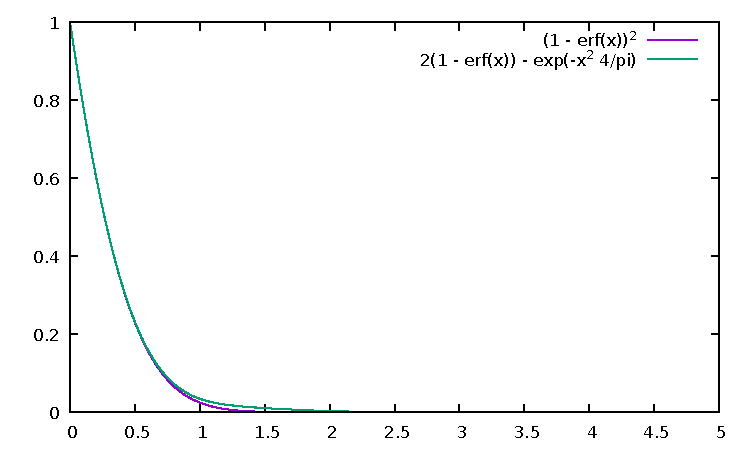
\includegraphics[width=1.00\linewidth]{fit_erf2.pdf}
        \caption{$\big(\text{erf}(x)\big)^2$ and its fit with $1 - e^{-\frac{4}{\pi} x^2}$.}
\end{figure*}

\bibliography{srDFT_SC}
\end{document}
